

%%% This LaTeX source document can be used as the basis for your technical
%%% report. Intentionally stripped and simplified
%%% and commands should be adjusted for your particular paper - title, 
%%% author, citations, equations, etc.
% % Citations/references are in report.bib 


\documentclass[conference,backref=page]{acmsiggraph}
\usepackage[toc,page]{appendix}
\usepackage{dblfloatfix}
\usepackage[]{algorithm2e}
\usepackage{graphicx}
\usepackage{booktabs}
\usepackage{float}
\usepackage{listings}
\usepackage{color}

\definecolor{dkgreen}{rgb}{0,0.6,0}
\definecolor{gray}{rgb}{0.5,0.5,0.5}
\definecolor{mauve}{rgb}{0.58,0,0.82}

\lstset{frame=tb,
	language=Java,
	aboveskip=3mm,
	belowskip=3mm,
	showstringspaces=false,
	columns=flexible,
	basicstyle={\small\ttfamily},
	numbers=none,
	numberstyle=\tiny\color{gray},
	keywordstyle=\color{blue},
	commentstyle=\color{dkgreen},
	stringstyle=\color{mauve},
	breaklines=true,
	breakatwhitespace=true,
	tabsize=3
}


\TOGonlineid{45678}
\TOGvolume{0}
\TOGnumber{0}
\TOGarticleDOI{1111111.2222222}
\TOGprojectURL{}
\TOGvideoURL{}
\TOGdataURL{}
\TOGcodeURL{}

% Include this so that citations show up in blue and the page information is included in the reference section
\hypersetup{
    colorlinks = true, 
    linkcolor = blue,
    anchorcolor = red,
    citecolor = blue, 
    filecolor = red, 
}


\title{Solving The Travelling Salesman Problem\\
	   A Report Analysing the Algorithms Used}

\author{Beej Persson\thanks{e-mail:40183743@live.napier.ac.uk} \\
Edinburgh Napier University\\
Algorithms and Data Structures (SET09117)}
\pdfauthor{Beej Persson}

\keywords{algorithms, data structures, travelling salesman, efficacy, efficiency, problem solving.}

\begin{document}

\maketitle

\raggedbottom

\begin{abstract}

The Travelling Salesman Problem is a common algorithmic problem often discussed in computer science. The problem itself is to find the shortest route of travel between all the desired cities without going to a city twice. This report looks to analyse two algorithmic solutions to this problem and compare them against each other. The first solution is the Nearest Neighbour algorithm whilst the second is a modified and enhanced version of that algorithm. Multiple tests were run to evaluate their efficacy, including measuring run time, comparing route lengths and increasing the number of cities.

\end{abstract}

\keywordlist

\section{Introduction}

\paragraph{The Problem}
Given a list of cities and their locations (and therefore the distances between each city), what is the shortest route from a starting city that travels to each city only once before returning to the starting city? Solving this problem is often not only about achieving the shortest possible route, there is a focus on optimisation: finding this shortest route in a reasonable time given the number of cities.

\paragraph{First Solution: Nearest Neighbour Basic}
The Nearest Neighbour algorithm used here solves the problem by starting with the first city in the file, checking the distances between it and all the other cities, picking the shortest distance then doing the same for that closest city with all the rest, whilst removing each previous city (this can be seen in Algorithm \ref{nnbasic} and in code in Appendix \ref{maincode}). This algorithm tends to return fairly short routes (although rarely the shortest) whilst also being fairly efficient. When used on a larger number of cities, the run time will still be comparatively low. This is due to it having an order of complexity of $n^2$, or $O(n^2)$, where the run time will increase in proportion to the problem size squared (for example the theoretical run time on a set of 10 cities will be 4 times bigger than on a set of 5, as $(10/5)^2 = 4$).

\begin{algorithm}[h]
	\caption{Nearest Neighbour Basic Psuedo-code}
	\label{nnbasic}
	\KwData{Array List of unsorted cities}
	\KwResult{Empty Array List (for sorted cities)}
	Point2D closest = null\;
	Point2D currentCity = Data.get(0)\;
	\While{cities.size \textgreater 0}{
		add currentCity to Result\;
		remove currentCity from Data\;
		distance = infinity\;
		\For{all city in Data}{
			\If{getDistance(currentCity to city) \textless distance}{
				closest = city\;
				distance = getDistance(currentCity to city)\;
			}
		}
		currentCity = closest\;
	}
	return Result\;
\end{algorithm}

\paragraph{Second Solution: Nearest Neighbour Enhanced}
The Nearest Neighbour Enhanced algorithm uses a fairly simple adaptation to the previous algorithm. Instead of starting with the first city in the file, it will start with a random city and find the closest city to it and carry on from there. After that it will calculate the length of that route. It will do these two steps a number of times (specifically a tenth of the number of cities in the file) and then look over the list of lengths and pick the lowest route length found (this can be seen in Algorithm \ref{nnenhanced} and in code in Appendix \ref{maincode}). This algorithm should consistently find lower route lengths at the expense of increased run time. As it is running the previous algorithm $n/10$ times (where n is the number of cities), its order of complexity is $O(n^3)$. This means that as the problem size increases, the run time will increase significantly (for example, the theoretical run time on a set of 10 cities will be 8 times bigger than on a set of 5, as $(10/5)^3 = 8$).

\begin{algorithm}[h]
	\caption{Nearest Neighbour Enhanced Psuedo-code}
	\label{nnenhanced}
	\KwData{Array List of unsorted cities}
	\KwResult{Empty Array List (for sorted cities)}
	Array List of Array Lists sortedCitiesList\;
	Array List lengths\;
	\For{int i \textless cities.size/10, i++}{
		Array List tempCitiesList = Data\;
		add nearestNeighbourRandomStart(tempCitiesList) to sortedCitiesList\;
		add routeLength(sortedCitiesList.get(i)) to legnths\;
		distance = infinity\;
		\If{lengths.get(i) \textless distance}{
			distance = lengths.get(i)\;
			Result = sortedCitiesList.get(i)\;
		}
	}
	return Result\;
\end{algorithm}

\section{Experimental Methods}

\paragraph{Overview}
The algorithms were tested against each other and on a variety of problem instances, with differing numbers of cities in each problem instance. The time it took the algorithm to return a sorted list of cities from the original unsorted list was used as the Run Time. The Route Length results were determined by calculating the length of the route between all the cities in the order of the sorted cities list. Tests were repeated for each algorithm for every problem instance. The results used in the later graphics were the averages of these repeated tests.

\paragraph{Detailed Description}
\begin{itemize}
\item {\bf Functionality of One Test}: Problem instance files containing a list of a certain number, $n$, of cities were loaded into an array list in Java. The algorithms sort this array list into an ordered list of cities, the order being the shortest route it found. The Run Time is calculated by finding the difference between the current time in milliseconds immediately before the algorithm is run and immediately after it returns a sorted list. This sorted list is then passed through a method that calculates the Route Length of the sorted cities in order. The Run Time and Route Length results were recorded for each test.
\item {\bf Testing Methodology}: For each of the chosen problem instances ten tests were run on each algorithm. For each test the results for the Run Time and the Route Length were then recorded in a table in an Excel file (see Figure \ref{exampletesttable}). The average Run Time and Route Length for each algorithm were stored in a separate table (Figure \ref{avgresultstable}) against the number of cities, $n$. This was the testing method used to produce the results and graphs analysed in this report.
\end{itemize}

\paragraph{Accuracy, Reliability and Reasoning for Testing Methodology}
 The number of cities in the file is initially known and is part of the file name. The number of cities in the array list (that the cities from the file are loaded into) is checked to match the number of cities in the file, and checked again after the algorithm is run. This is to ensure that the Route Length for the shortest route found is including every city in the problem instance and eliminate any artificially short routes. Nine problem instances were used, with an appropriately varying number of cities in each (ranging from 52 cities, up to 5915 cities) to help visualise the effect of $n$ on the Run Time of the two algorithms. Each problem instance tested stored the location of cities as points in Euclidean 2D geometry (with $x$, $y$ coordinates) and the way the software loaded the file's city list into an array list relied upon the city locations being stored this way. Therefore only problem instances that stored the cities in this way were tested. The Run Time results were recorded in milliseconds to best represent the time taken, with a problem instance with a small number of cities taking only a few milliseconds, and larger sample sizes taking hundreds and even thousands of milliseconds. Seconds could also have been chosen and been similarly effective due to the wide range of times achieved. The Route Length results were recorded with arbitrary units, as the location of each city was simply stored as a 2D point in the files with no indication of the units of the $x$ and $y$ coordinates. Each test was run on the same PC, from the same code, with each result being recorded one at a time to reduce memory build up slowing down Run Time and improve the accuracy and repeatability of the results. Ten tests were run for each problem instance and for each algorithm and the average Run Times and Route Lengths were used for displaying the results to further improve reliability of the accuracy of the testing methodology.


\section{Results}

\paragraph{Tables}
\begin{figure}[h]
	\begin{center}
		\resizebox{\columnwidth}{!}{%
		\begin{tabular}{@{}r|cccc@{}}
			\toprule
			\multicolumn{1}{l}{} & \multicolumn{4}{c}{u1060.tsp -\textgreater n = 1060} \\ \midrule
			\multicolumn{1}{l|}{} & \multicolumn{2}{c|}{Nearest Neighbour Basic} & \multicolumn{2}{c}{Nearest Neighbour Enhanced} \\ \midrule
			\multicolumn{1}{c|}{Test} & \multicolumn{1}{c|}{Time / ms} & \multicolumn{1}{c|}{Route Length / units} & \multicolumn{1}{c|}{Time / ms} & Route Length / units \\ \midrule
			1 & 13 & \multicolumn{1}{c|}{296,543.889} & 1,095 & 282,301.279 \\
			2 & 14 & \multicolumn{1}{c|}{296,543.889} & 1,104 & 281,639.607 \\
			3 & 13 & \multicolumn{1}{c|}{296,543.889} & 1,109 & 281,581.385 \\
			4 & 14 & \multicolumn{1}{c|}{296,543.889} & 1,103 & 281,006.855 \\
			5 & 13 & \multicolumn{1}{c|}{296,543.889} & 1,103 & 281,581.385 \\
			6 & 13 & \multicolumn{1}{c|}{296,543.889} & 1,103 & 281,006.855 \\
			7 & 13 & \multicolumn{1}{c|}{296,543.889} & 1,109 & 281,329.829 \\
			8 & 13 & \multicolumn{1}{c|}{296,543.889} & 1,093 & 281,444.456 \\
			9 & 14 & \multicolumn{1}{c|}{296,543.889} & 1,099 & 282,083.731 \\
			10 & 13 & \multicolumn{1}{c|}{296,543.889} & 1,106 & 281,329.829 \\ \midrule
			Avg & 13.3 & \multicolumn{1}{c|}{296,543.889} & 1,102.4 & 281,530.521 \\ \bottomrule
		\end{tabular}%
		}
		\caption{The table produced from the results of ten tests run for each algorithm on the file u1060.tsp, where $n$ is the number of cities which equals 1060.}
		\label{exampletesttable}
	\end{center}
\end{figure}

Figure \ref{exampletesttable} shows an example table of the testing. The problem instance file name and the number of cities in that file is at the top and the test number that the results correspond to are on the left. The results for both algorithms were stored in the same table in separate columns and the averages of the results are shown at the bottom of the table. The Run Time results were recorded to the nearest millisecond, whereas Route Length was to three decimal places. A table similar to this was produced for all nine problem instances and an averages table (see Figure \ref{avgresultstable}) was produced from the averages of the results from each test of the algorithms on the separate problem instances. For some comparisons made later, a ratios table (see Figure \ref{ratioresultstable}) was also produced by deriving the ratio of the Enhanced algorithm's results compared to the Basic algorithm's. Shown to the right is that final averages table.

\begin{figure}[h]
	\begin{center}
		\resizebox{\columnwidth}{!}{%
			\begin{tabular}{@{}rcccc@{}}
				\toprule
				\multicolumn{1}{l}{} & \multicolumn{4}{c}{Averages} \\ \midrule
				\multicolumn{1}{l|}{} & \multicolumn{2}{c|}{Nearest Neighbour Basic} & \multicolumn{2}{c}{Nearest Neighbour Enhanced} \\ \midrule
				\multicolumn{1}{c|}{n} & \multicolumn{1}{c|}{Time / ms} & \multicolumn{1}{c|}{Route Length / units} & \multicolumn{1}{c|}{Time / ms} & Route Length / units \\ \midrule
				\multicolumn{1}{r|}{52} & 0.6 & \multicolumn{1}{c|}{8,980.92} & 1.0 & 8,883.10 \\
				\multicolumn{1}{r|}{101} & 1.0 & \multicolumn{1}{c|}{825.24} & 2.5 & 759.50 \\
				\multicolumn{1}{r|}{159} & 1.6 & \multicolumn{1}{c|}{54,669.03} & 5.6 & 50,251.97 \\
				\multicolumn{1}{r|}{262} & 5.8 & \multicolumn{1}{c|}{3,241.47} & 19.9 & 2,920.33 \\
				\multicolumn{1}{r|}{493} & 4.9 & \multicolumn{1}{c|}{43,646.37} & 125.0 & 41,982.41 \\
				\multicolumn{1}{r|}{1060} & 13.3 & \multicolumn{1}{c|}{296,543.89} & 1,102.4 & 281,530.52 \\
				\multicolumn{1}{r|}{2103} & 44.2 & \multicolumn{1}{c|}{90,517.89} & 8,113.1 & 87,664.57 \\
				\multicolumn{1}{r|}{3795} & 137.1 & \multicolumn{1}{c|}{35,362.51} & 45,949.0 & 34,226.09 \\
				\multicolumn{1}{r|}{5915} & 336.4 & \multicolumn{1}{c|}{707,498.63} & 179,763.5 & 672,798.03 \\ \bottomrule
			\end{tabular}%
		}
		\caption{The Table of Averages produced by averaging all the results from the tests, where $n$ is the number of cities.}
		\label{avgresultstable}
	\end{center}
\end{figure}

The averages table has the problem instances' number of cities, $n$, on the left with the corresponding averages of the test results for each algorithm displayed in the neighbouring columns. The Run Times were recorded to one decimal place in milliseconds and the Route Length to the nearest two decimal places. This was to tidy the table up from the test tables.

\begin{figure}[H]
	\begin{center}
		\resizebox{\columnwidth}{!}{%
			\begin{tabular}{@{}rcccc@{}}
				\toprule
				\multicolumn{1}{l}{} & \multicolumn{4}{c}{Ratios} \\ \midrule
				\multicolumn{1}{l|}{} & \multicolumn{2}{c|}{Nearest Neighbour Basic} & \multicolumn{2}{c}{Nearest Neighbour Enhanced} \\ \midrule
				\multicolumn{1}{c|}{n} & \multicolumn{1}{c|}{Time} & \multicolumn{1}{c|}{Route Length} & \multicolumn{1}{c|}{Time} & \multicolumn{1}{c}{Route Length} \\ \midrule
				\multicolumn{1}{r|}{52} & 1.0 & \multicolumn{1}{c|}{1.0} & 1.7 & 0.989 \\
				\multicolumn{1}{r|}{101} & 1.0 & \multicolumn{1}{c|}{1.0} & 2.5 & 0.920 \\
				\multicolumn{1}{r|}{159} & 1.0 & \multicolumn{1}{c|}{1.0} & 3.5 & 0.919 \\
				\multicolumn{1}{r|}{262} & 1.0 & \multicolumn{1}{c|}{1.0} & 3.4 & 0.901 \\
				\multicolumn{1}{r|}{493} & 1.0 & \multicolumn{1}{c|}{1.0} & 25.5 & 0.962 \\
				\multicolumn{1}{r|}{1060} & 1.0 & \multicolumn{1}{c|}{1.0} & 82.9 & 0.949 \\
				\multicolumn{1}{r|}{2103} & 1.0 & \multicolumn{1}{c|}{1.0} & 183.6 & 0.968 \\
				\multicolumn{1}{r|}{3795} & 1.0 & \multicolumn{1}{c|}{1.0} & 335.1 & 0.968 \\
				\multicolumn{1}{r|}{5915} & 1.0 & \multicolumn{1}{c|}{1.0} & 534.4 & 0.951 \\ \bottomrule
			\end{tabular}%
		}
		\caption{The Table of Ratios shows how the Nearest Neighbour Enhanced algorithm compares to the Basic algorithm by seeing the results as a ratio of each other.}
		\label{ratioresultstable}
	\end{center}
\end{figure}

The ratios table has the problem instances' number of cities, $n$, on the left with the corresponding ratios for each algorithm displayed in the neighbouring columns. The Run Times and the Route Length results of both the algorithms were divided by the Basic algorithm's results to find the ratios shown.


\paragraph{Efficacy Graphs}
The graph shown below (Figure \ref{efficacycomparedcolumngraph}) displays the results found for the Route Length for the shortest route found by both the Nearest Neighbour Basic and Nearest Neighbour Enhanced algorithms against the separate problem instances (a full size version is found in Appendix \ref{efficacycomparedgraph}). For every problem instance tested the Enhanced algorithm achieved a shorter Route Length than the basic algorithm. However this graph has some results as low as $759.5$ units (for $n = 101$) and as high as $707,498.6$ units (for $n = 5915$), therefore it's hard to display by how much the Enhanced algorithm improved upon the shortest route found by the Basic algorithm for some of the problem instances tested.

\begin{figure}[h]
	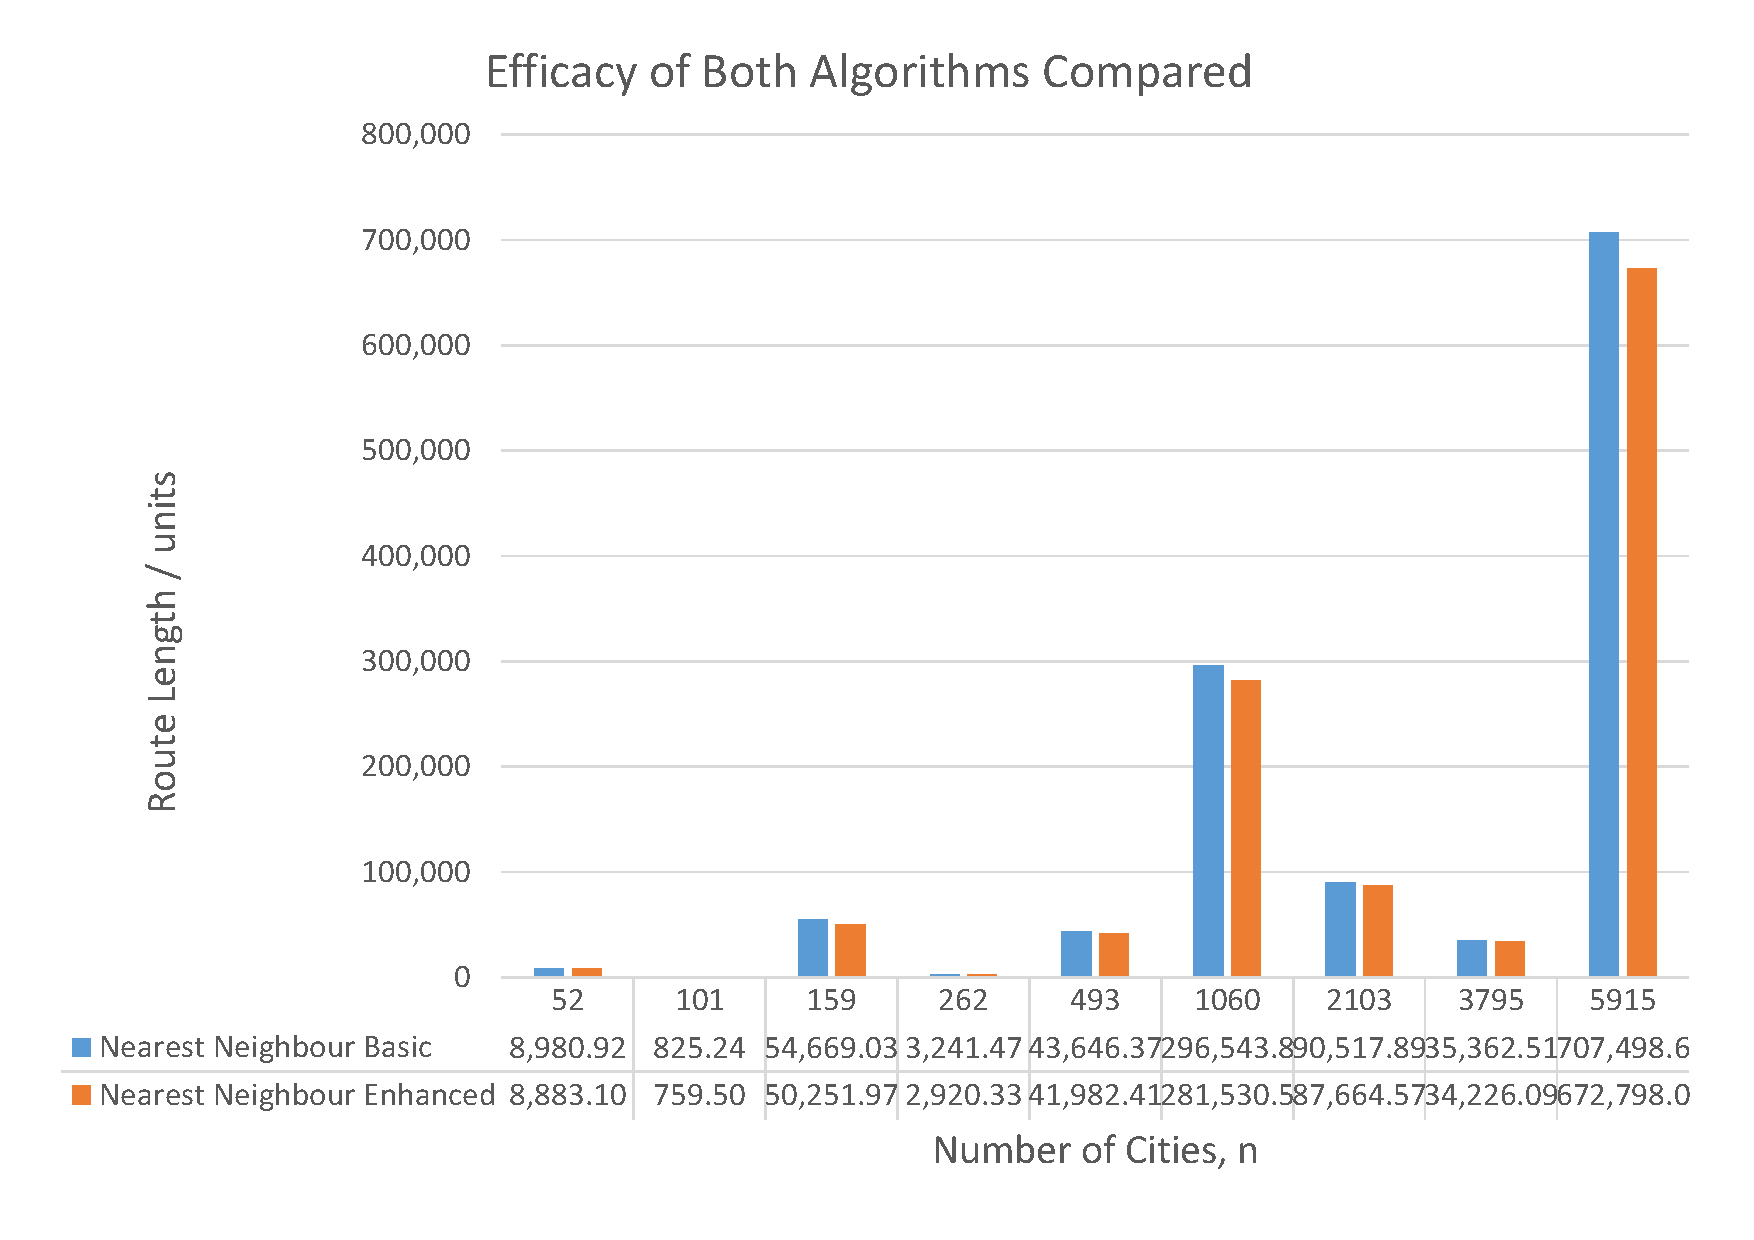
\includegraphics[width=\columnwidth]{images/efficacy_compared_column.pdf}
	\caption{A graph showing how the average Route Length results of both algorithms compared for the differing number of cities in each problem instance.}
	\label{efficacycomparedcolumngraph}
\end{figure}

 A similar graph (show below in Figure \ref{efficacycomparedratioscolumngraph} and in full in Appendix \ref{efficacycomparedratiosgraph}) that showed the Route Length found by the Enhanced algorithm as a ratio of what was found by the Basic algorithm was used to help better display this. Here it is clear that even for smaller data sets (where the Route Length tended to be fairly small also) the Enhanced algorithm was still consistently finding shorter routes. In fact, for the two problem instances that are almost invisible on Figure \ref{efficacycomparedcolumngraph} ($n = 101$ and $n = 262$), the Enhanced algorithm returned a proportionally shorter route than it did on the larger data sets when compared against the Basic algorithm.

\begin{figure}[H]
	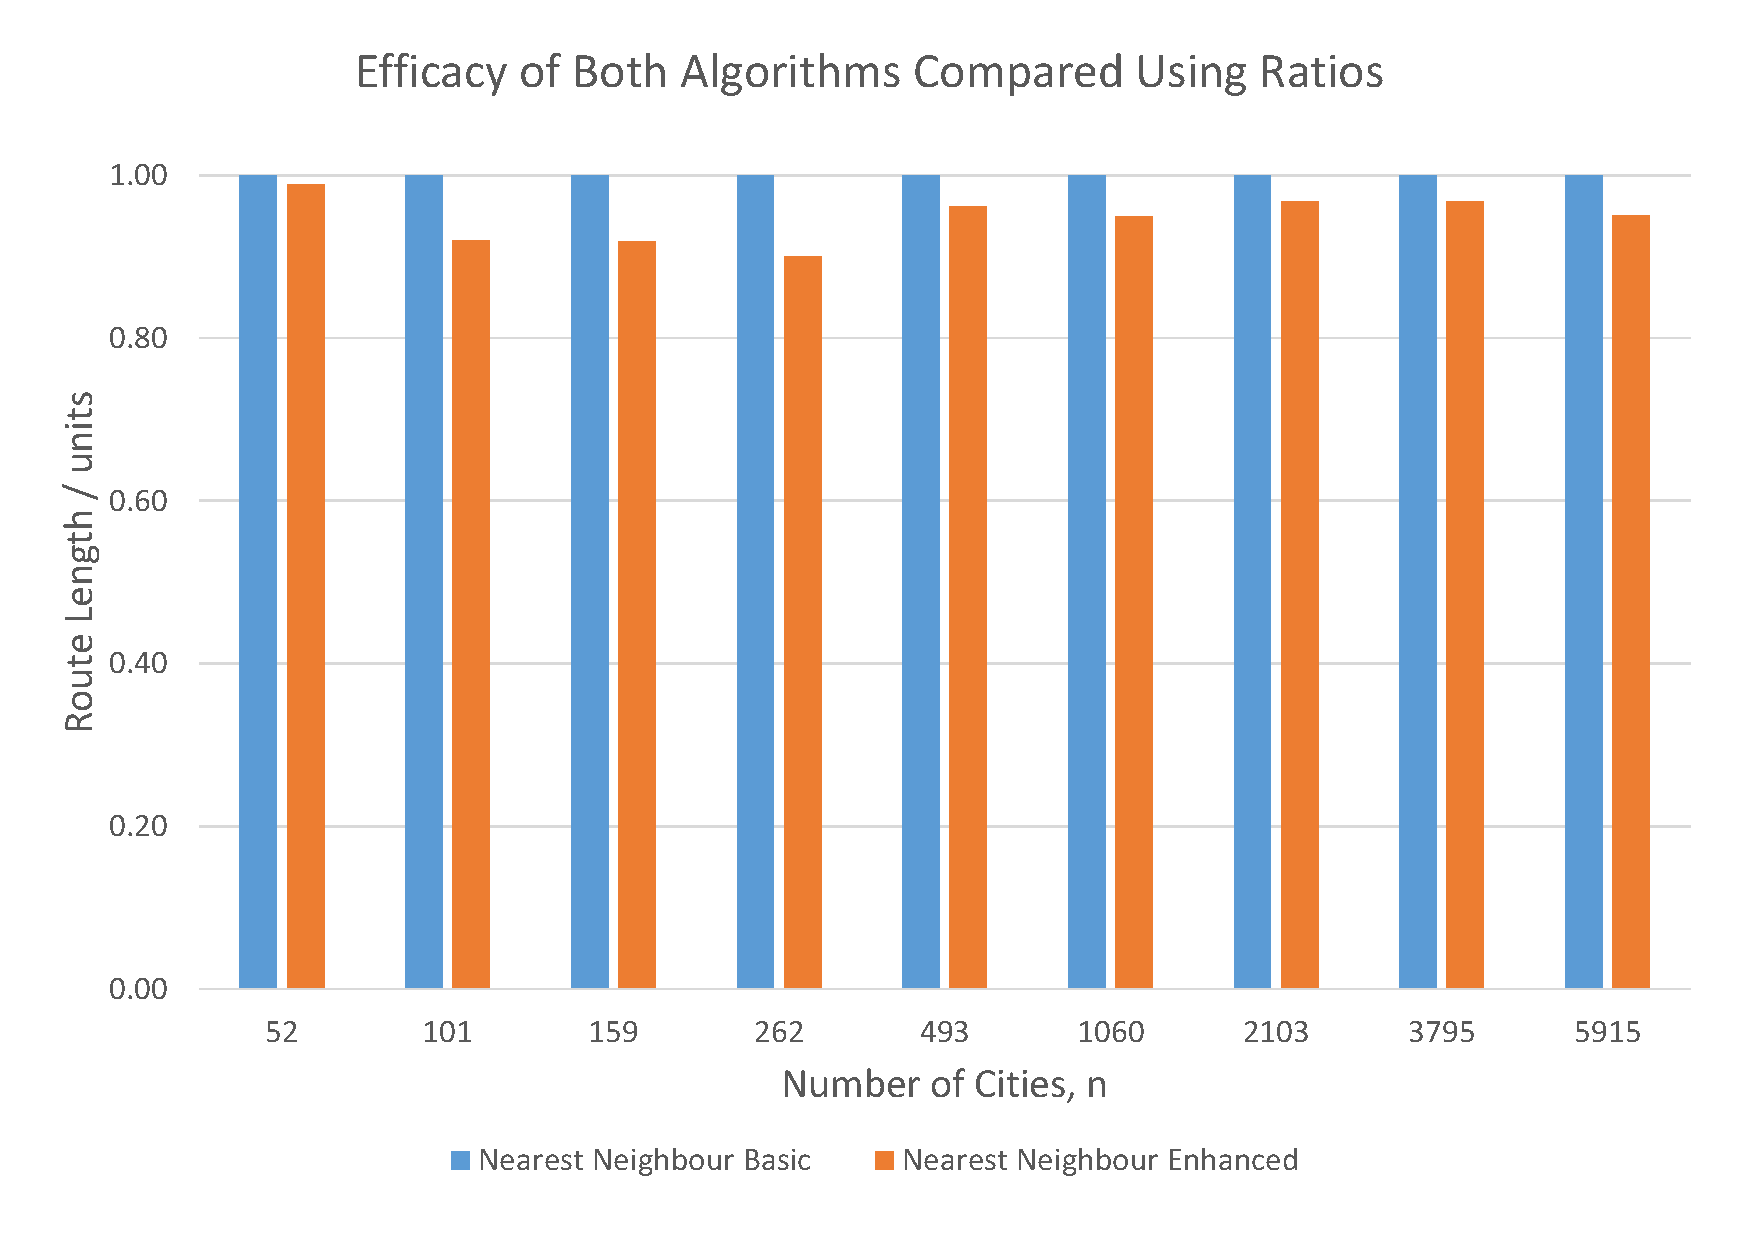
\includegraphics[width=\columnwidth]{images/efficacy_compared_ratios_column.pdf}
	\caption{A graph showing the Enhanced algorithm's average Route Length results as a ratio of the Basic algorithm's results.}
	\label{efficacycomparedratioscolumngraph}
\end{figure}

\paragraph{Efficiency Graphs}
Whilst it's important for an algorithm that solves the Travelling Salesman Problem to return a short route, the time it takes for the algorithm to complete the task must be taken into account, especially when considering problem instances with very large numbers of cities. The graph shown below (Figure \ref{efficiencybasiccolumngraph}) displays the Run Time results of the Nearest Neighbour Basic algorithm against the Number of Cities, $n$, of the separate problem instances (a full size version is found in Appendix \ref{efficiencybasicgraph}). As mentioned earlier, the Basic algorithm has complexity $O(n^2)$, this is reinforced by the results displayed below. A polynomial trendline of order 2 has been generated for the data that shows this. The average Run Time results clearly increase proportional to the increase in the Number of Cities, $n$, squared. However, this algorithm is still returning solutions to the problem fairly fast. For seven of the nine problem instances tested the Basic algorithm solved the problem and returned a route in less than $50ms$. Whilst the other two problem instances take up to $350ms$, this is still very quick, especially when compared to the Enhanced algorithm's Run Time results, shown below.

\begin{figure}[h]
	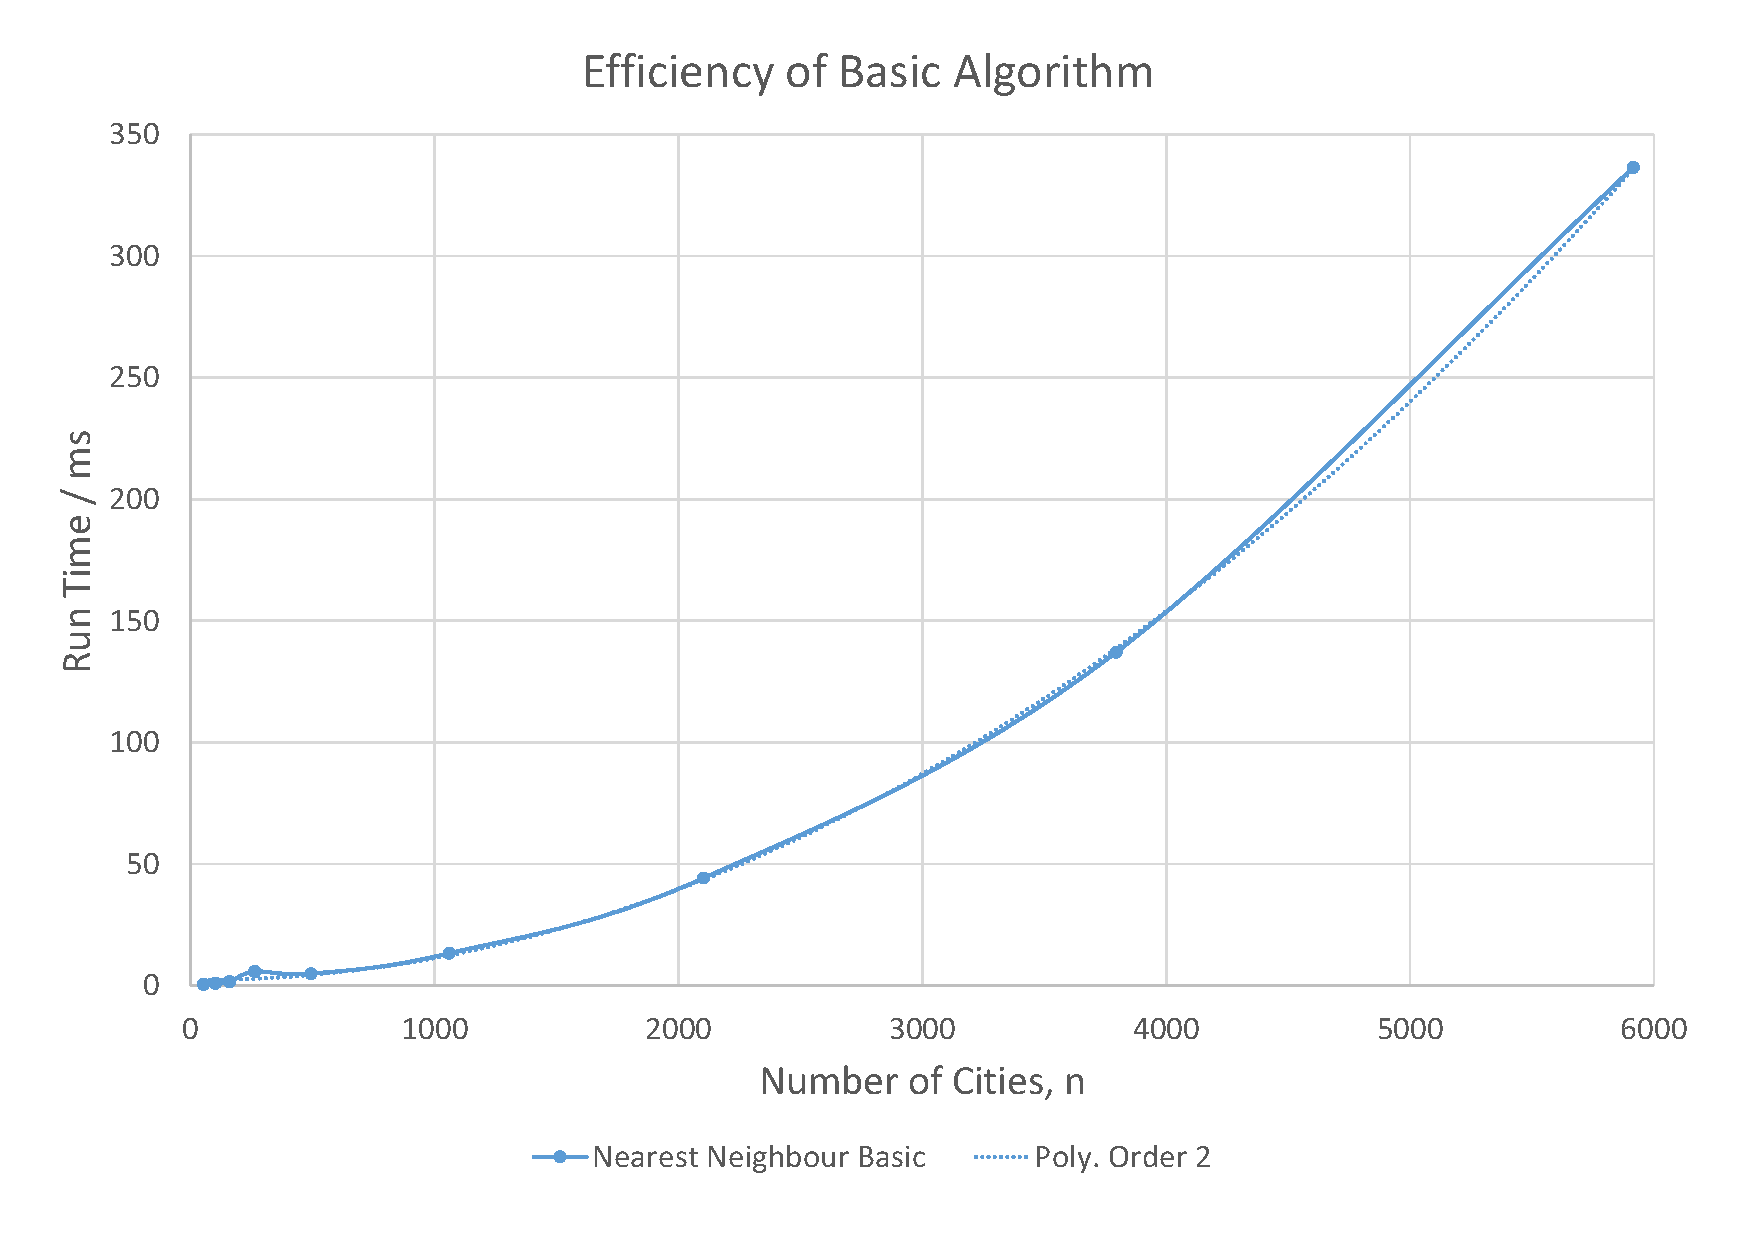
\includegraphics[width=\columnwidth]{images/efficiency_basic_column.pdf}
	\caption{A graph showing the Nearest Neighbour Basic algorithm's average Run Time compared against the number of cities in each problem instance. The trendline is a polynomial trendline of order 2, aligning with the algorithm's order of complexity.}
	\label{efficiencybasiccolumngraph}
\end{figure}

The Nearest Neighbour Enhanced algorithm consistently found shorter Route Lengths when solving the same problem instances as the Basic algorithm. However, the average Run Time results for each test very quickly got significantly higher than the Basic algorithm's Run Time results. Shown below (in Figure \ref{efficiencyenhancedcolumngraph}) is a graph that displays the efficiency of the Enhanced algorithm, putting it's Run Time against the Number of Cities, $n$, in the problem instances it was tested on (a full size graph can be found in Appendix \ref{efficiencyenhancedgraph}). The Enhanced algorithm has complexity $O(n^3)$ as it iterates through a tenth of the total number of cities performing the Nearest Neighbour Random Start algorithm (complexity $O(n^2)$) each time. This is shown by the polynomial trendline of order 3 generated from the data displayed on the graph. Because of this the average Run Time results are very high, especially for medium and larger data sets. Only for problem instances with less than around $500$ cities did the Enhanced algorithm run in less than $200ms$, and beyond this Run Times start increasing even further. For the two problem instances with the largest number of cities the Enhanced algorithm returns a shortest route in roughly $46$ and $180$ seconds respectively (specifically $45,949.0ms$ and $179,763.5ms$). Because of this, the two algorithms' Run Time results are poorly displayed on a graph with a linear scaled Run Time axis, as the results of the Enhanced algorithm dwarf the other results. Therefore a graph with a logarithmic scale is used to show the significant difference between the efficiency of both algorithms.

\begin{figure}[h]
	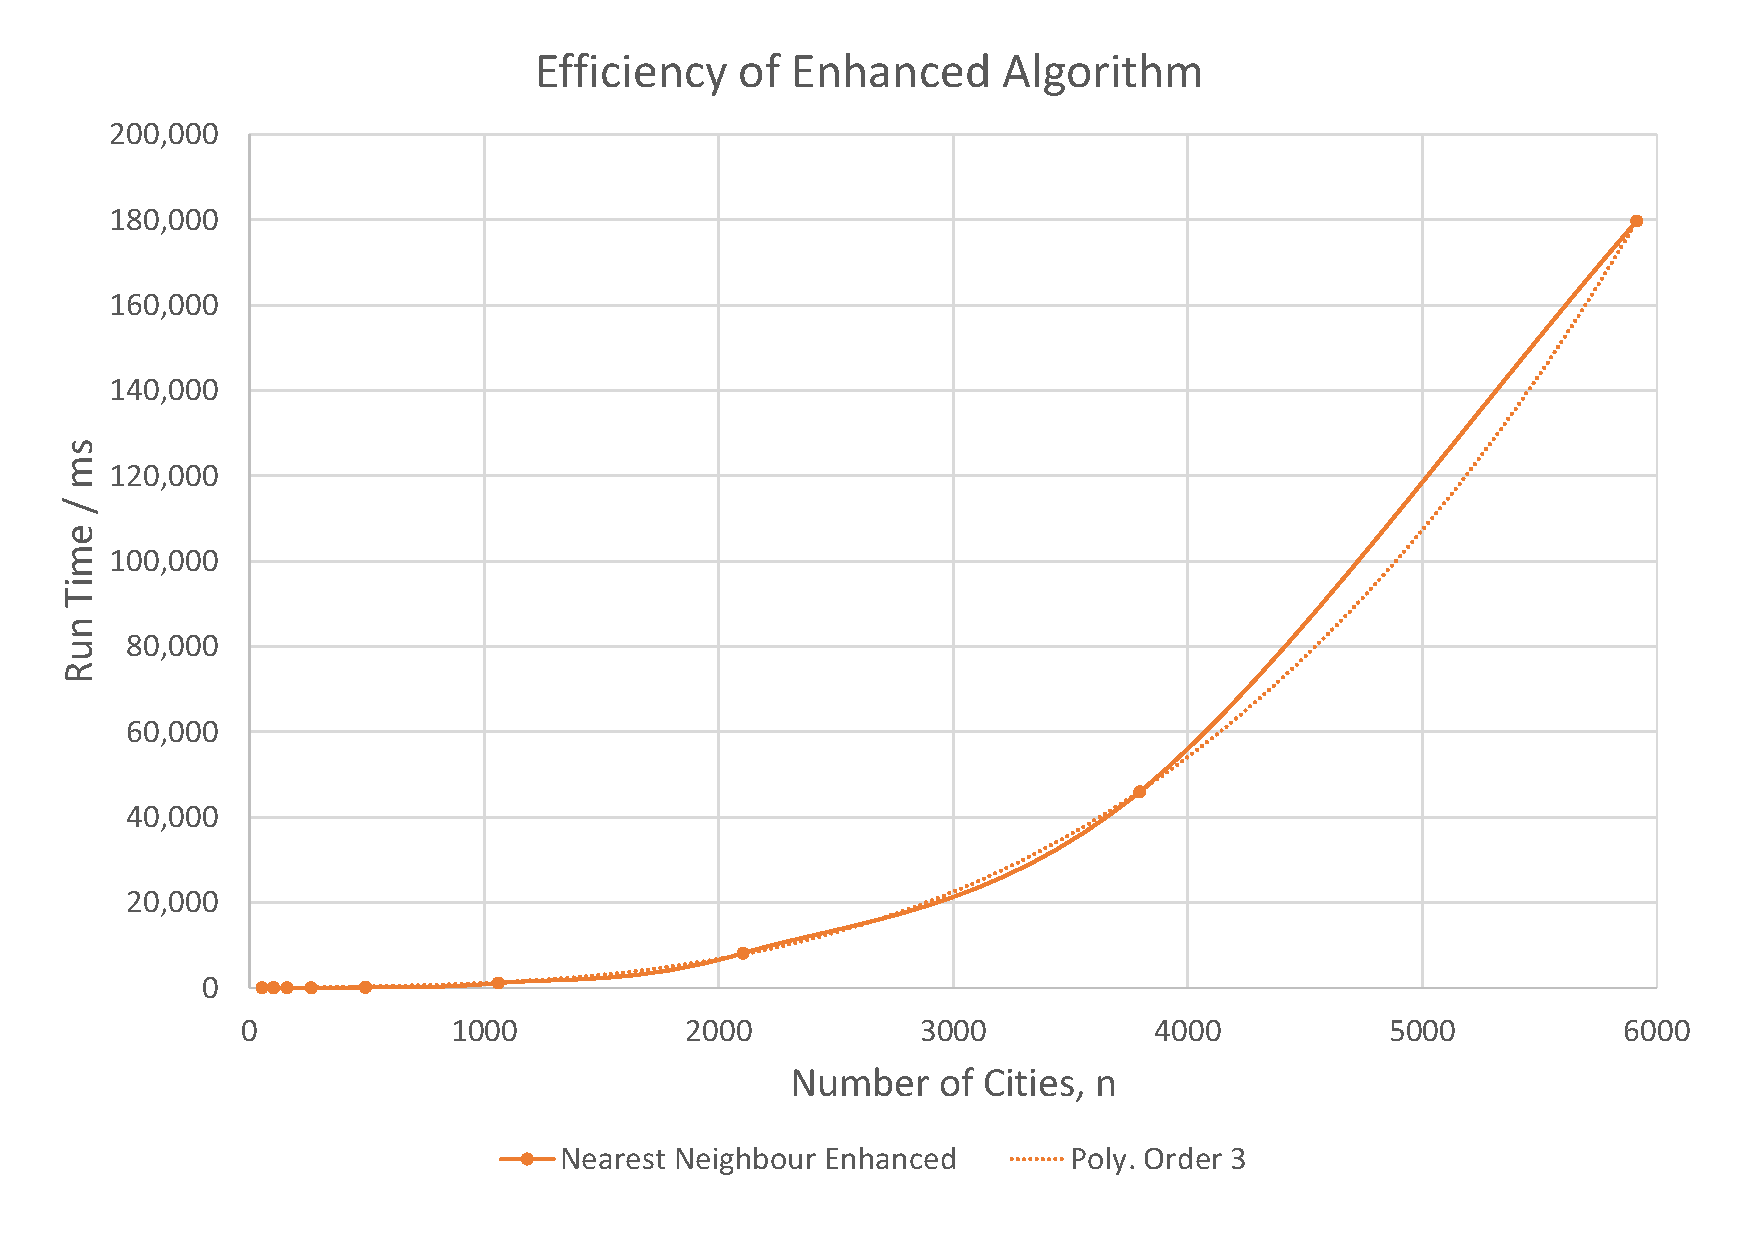
\includegraphics[width=\columnwidth]{images/efficiency_enhanced_column.pdf}
	\caption{A graph showing the Nearest Neighbour Enhanced algorithm's average Run Time compared against the number of cities in each problem instance. The trendline is a polynomial trendline of order 3, aligning with the algorithm's order of complexity.}
	\label{efficiencyenhancedcolumngraph}
\end{figure}

The graph below (Figure \ref{efficiencycomparedcolumngraph}) shows the comparison between both the algorithms' Run Times on a logarithmic scale (a full sized graph can be found in Appendix \ref{efficiencycomparedgraph}). Once again for both the Enhanced and Basic algorithms there are generated polynomial trendlines of order 2 and 3 respectively shown in the graph that reinforce the separate algorithms' order of complexity, as discussed earlier. Using this graph it is clear that whilst the Enhanced algorithm regularly returns shorter final route lengths, the Basic algorithm finds the solution significantly faster. On smaller data sets (up to 500 cities) the difference in time is negligible (within one tenth of a second), but as the number of cities in the problem instance increases, the Run Time for the Enhanced algorithm becomes large enough to become a problem. The largest data set tested had 5915 cities, for this problem the Basic algorithm returned a Route Length in an average Run Time of $336.4ms$, whereas the Enhanced algorithm returned a Route Length in an average Run Time of $179.763.5ms$, or roughly 3 minutes. Given a data set of 10,000 or more cities, using the Enhanced algorithm to solve the problem becomes increasingly infeasible. 

\begin{figure}[h]
	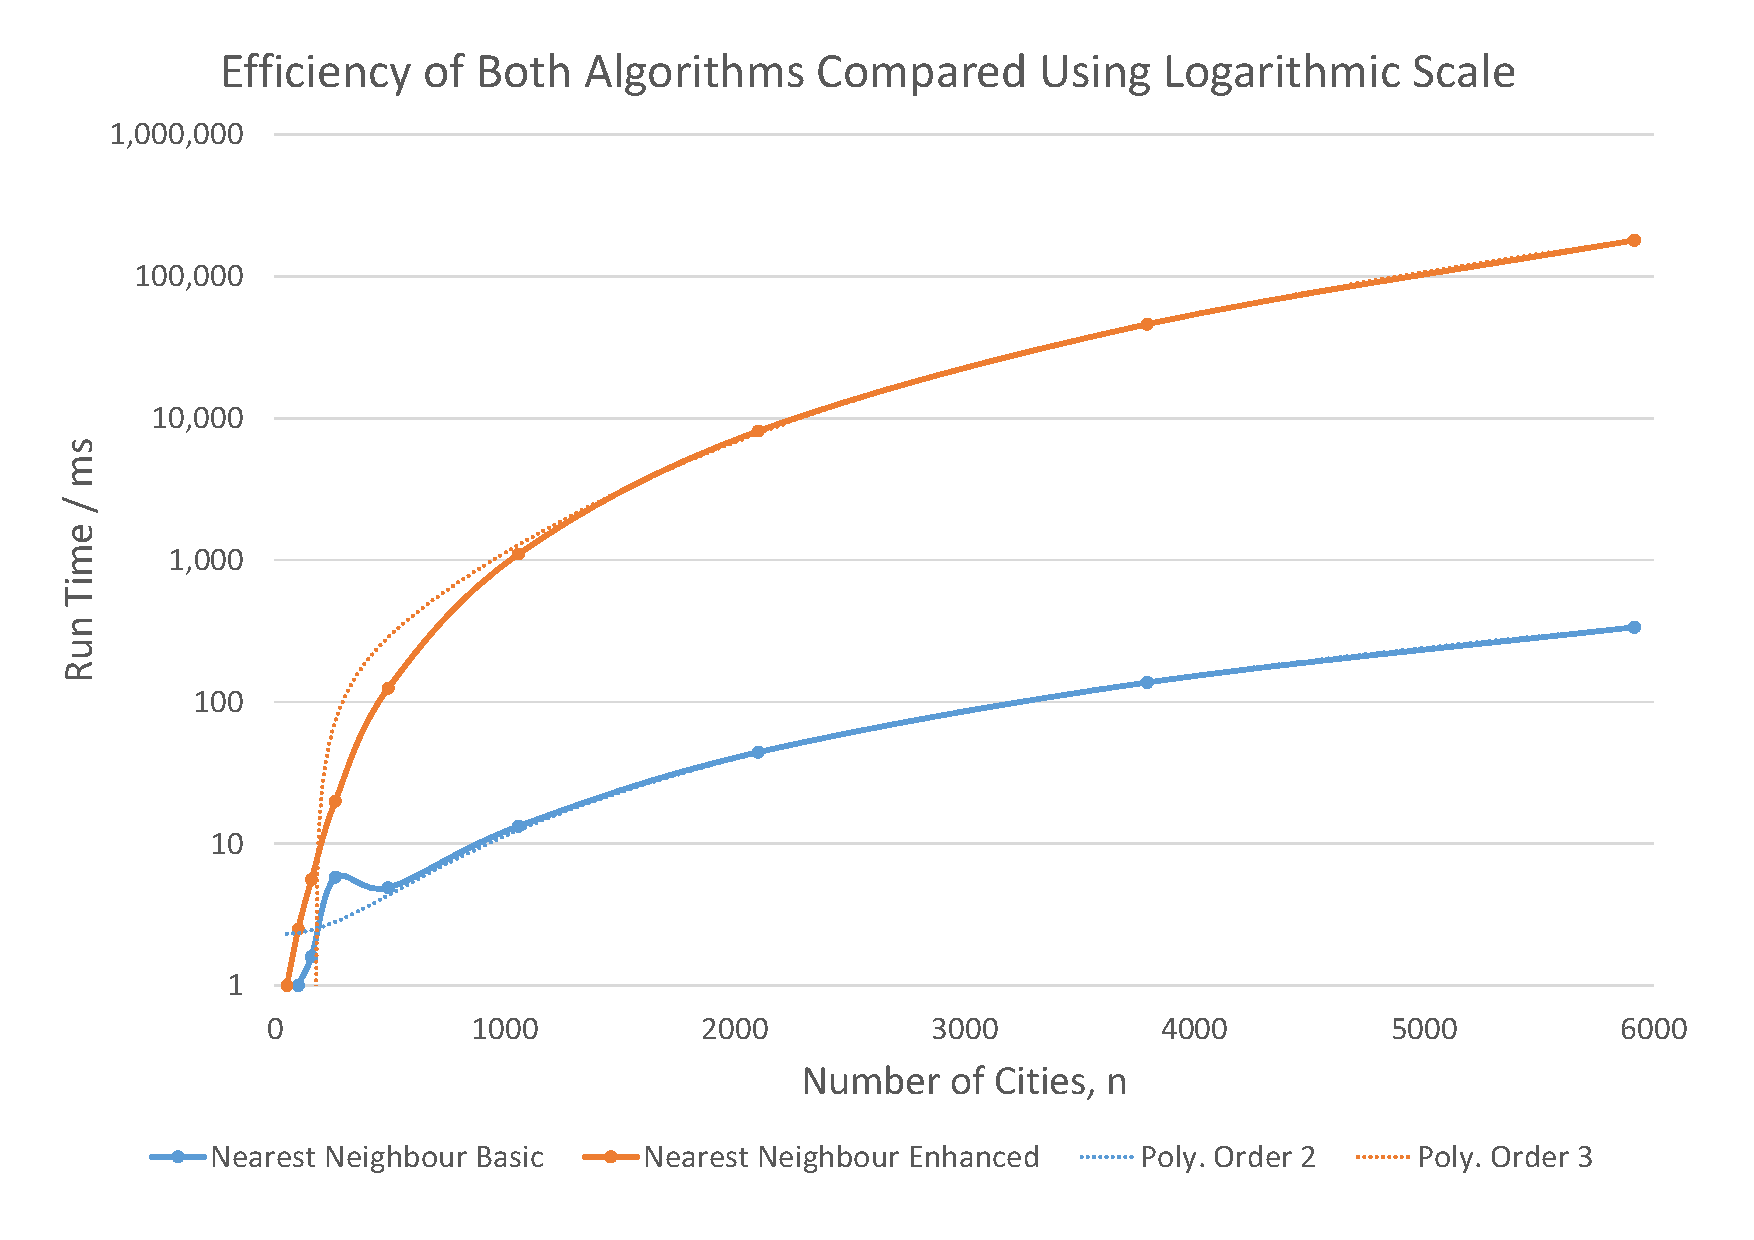
\includegraphics[width=\columnwidth]{images/efficiency_compared_column.pdf}
	\caption{A graph showing the Nearest Neighbour Basic algorithm's average Run Time compared with the Nearest Neighbour Enhanced algorithm's average Run Time against the number of cities in each problem instance using a logarithmic scale. The trendlines are polynomial trendlines of order 2 and 3 respectively.}
	\label{efficiencycomparedcolumngraph}
\end{figure}

\section{Conclusions}
\paragraph{Results Explanations}
The Nearest Neighbour Basic algorithm finds the shortest route that visits each city only once from a list of unsorted cities by finding the closest city to the first city in the list, then finding the closest city to that city and does this for all cities in the list (refer to Algorithm \ref{nnbasic} and Appendix \ref{maincode}). It has an order of complexity of $O(n^2)$, where $n$ is the number of cities in the unsorted list, as for each city in the list it looks at the distance between it and all other cities. Because of this the time it takes for the algorithm to return a solution will be proportional to the number of cities in the list squared. The Nearest Neighbour Enhanced algorithm, however, finds the shortest route by running an adapted version of the Basic algorithm, where it starts with a random city in the unsorted list as opposed to the first city, multiple (a tenth of $n$) times, and choosing the shortest route out of all the routes found (refer to Algorithm \ref{nnenhanced} and Appendix \ref{maincode}). Because of this the order of complexity is $n^2 \times n/10$ or $O(n^3)$. Due to having a wide range of routes, found by running the adapted Nearest Neighbour algorithm multiple times, to select the lowest Route Length from; the Enhanced algorithm reliably produces a final solution to the problem with a shorter Route Length than the Basic algorithm (as seen in Figures \ref{efficacycomparedcolumngraph} and \ref{efficacycomparedratioscolumngraph} (Appendix \ref{efficacycomparedgraph} and \ref{efficacycomparedratiosgraph} respectively)). However, as stated before, finding a shorter route comes at a cost. The effect of the increased complexity can clearly be seen in Figures \ref{efficiencybasiccolumngraph}, \ref{efficiencyenhancedcolumngraph} and \ref{efficiencycomparedcolumngraph} (Appendix \ref{efficiencybasicgraph}, \ref{efficiencyenhancedgraph} and \ref{efficiencycomparedgraph} respectively or full size graphs). The Run Time results for the Enhanced algorithm are longer than the Basic algorithm's for all data sets and significantly so when the number of cities becomes larger.
\paragraph{Reflections on the Value of the Algorithms}
There were many parameters put in place to ensure accuracy and repeatability of the tests, for example the Run Time was calculated looking only at the time it took for the algorithm to return a sorted list and there were multiple tests done for multiple problem instances, all done on the same PC. Given these parameters and that the results represented what was expected of the algorithms due to their respective orders of complexity, the results can be said to be reliable, therefore the values of the separate algorithms can be discussed. It is clear that the Nearest Neighbour Enhanced algorithm repeatedly found shorter routes for every problem instance tested, and that for smaller data sets it did this with a negligible increase in Run Time. However, for how much shorter the route found was compared to what the Basic algorithm found, the increase in the Run Time becomes increasingly hard to justify for larger data sets. Referring to the ratios table, Figure \ref{ratioresultstable}, it is clear that for problem instances with more than 500 cities the Run Time is hundreds of times larger, whilst the Route Length found is still only, at best, 0.95 times what the Basic algorithm found.
\paragraph{Final Thoughts}
The increase from an order of complexity of $O(n^2)$ to $O(n^3)$ will significantly increase the Run Time for large values of $n$. As such, given the negligible improvement in the length of the route found by the Enhanced algorithm, for any Travelling Salesman Problem instances the Enhanced algorithm should only be preferred for instances with a comparatively small numbers of cities, otherwise the Basic algorithm is superior.

\clearpage
\begin{appendices}
	\section{Efficacy Compared}
		\label{efficacycomparedgraph}
		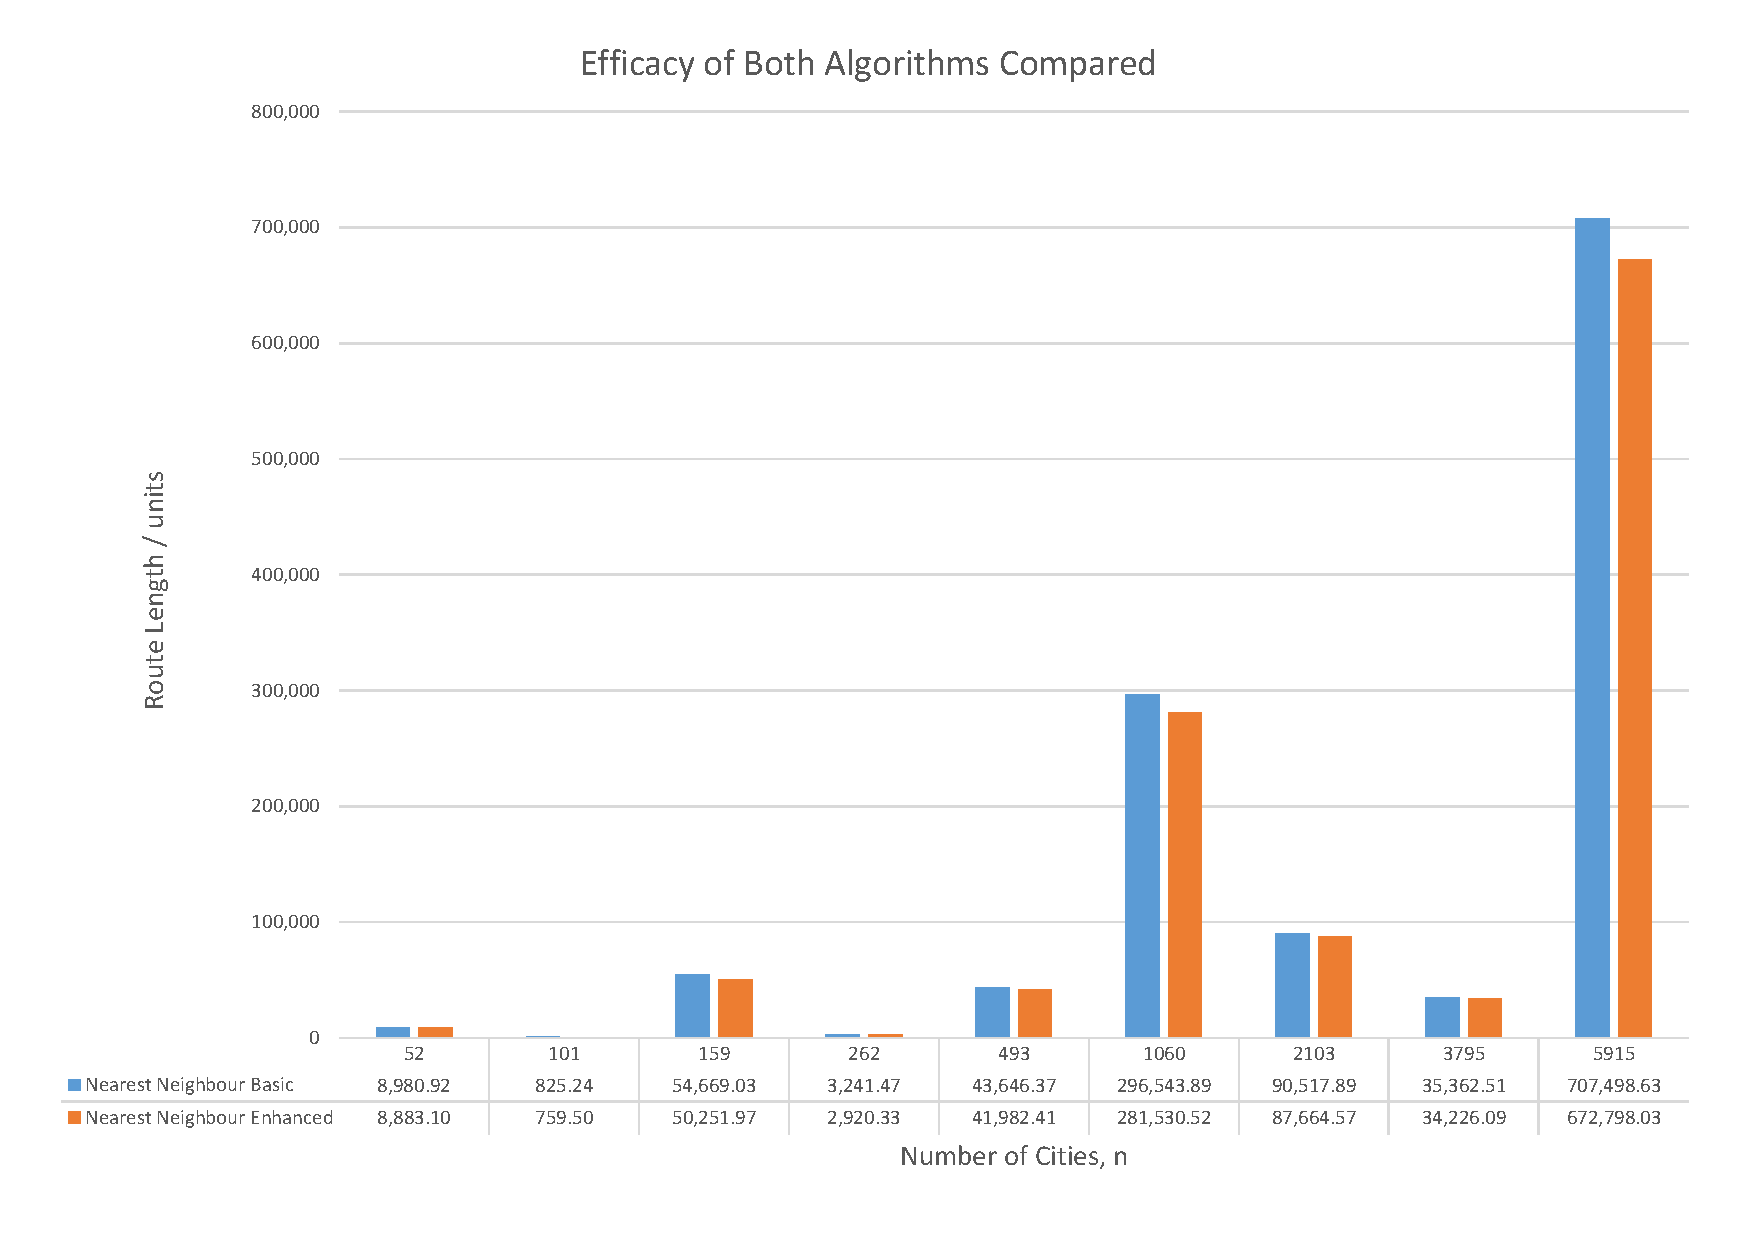
\includegraphics[width=\textwidth]{images/efficacy_compared.pdf}
	\clearpage
	\section{Efficacy Compared Using Ratios}
		\label{efficacycomparedratiosgraph}
		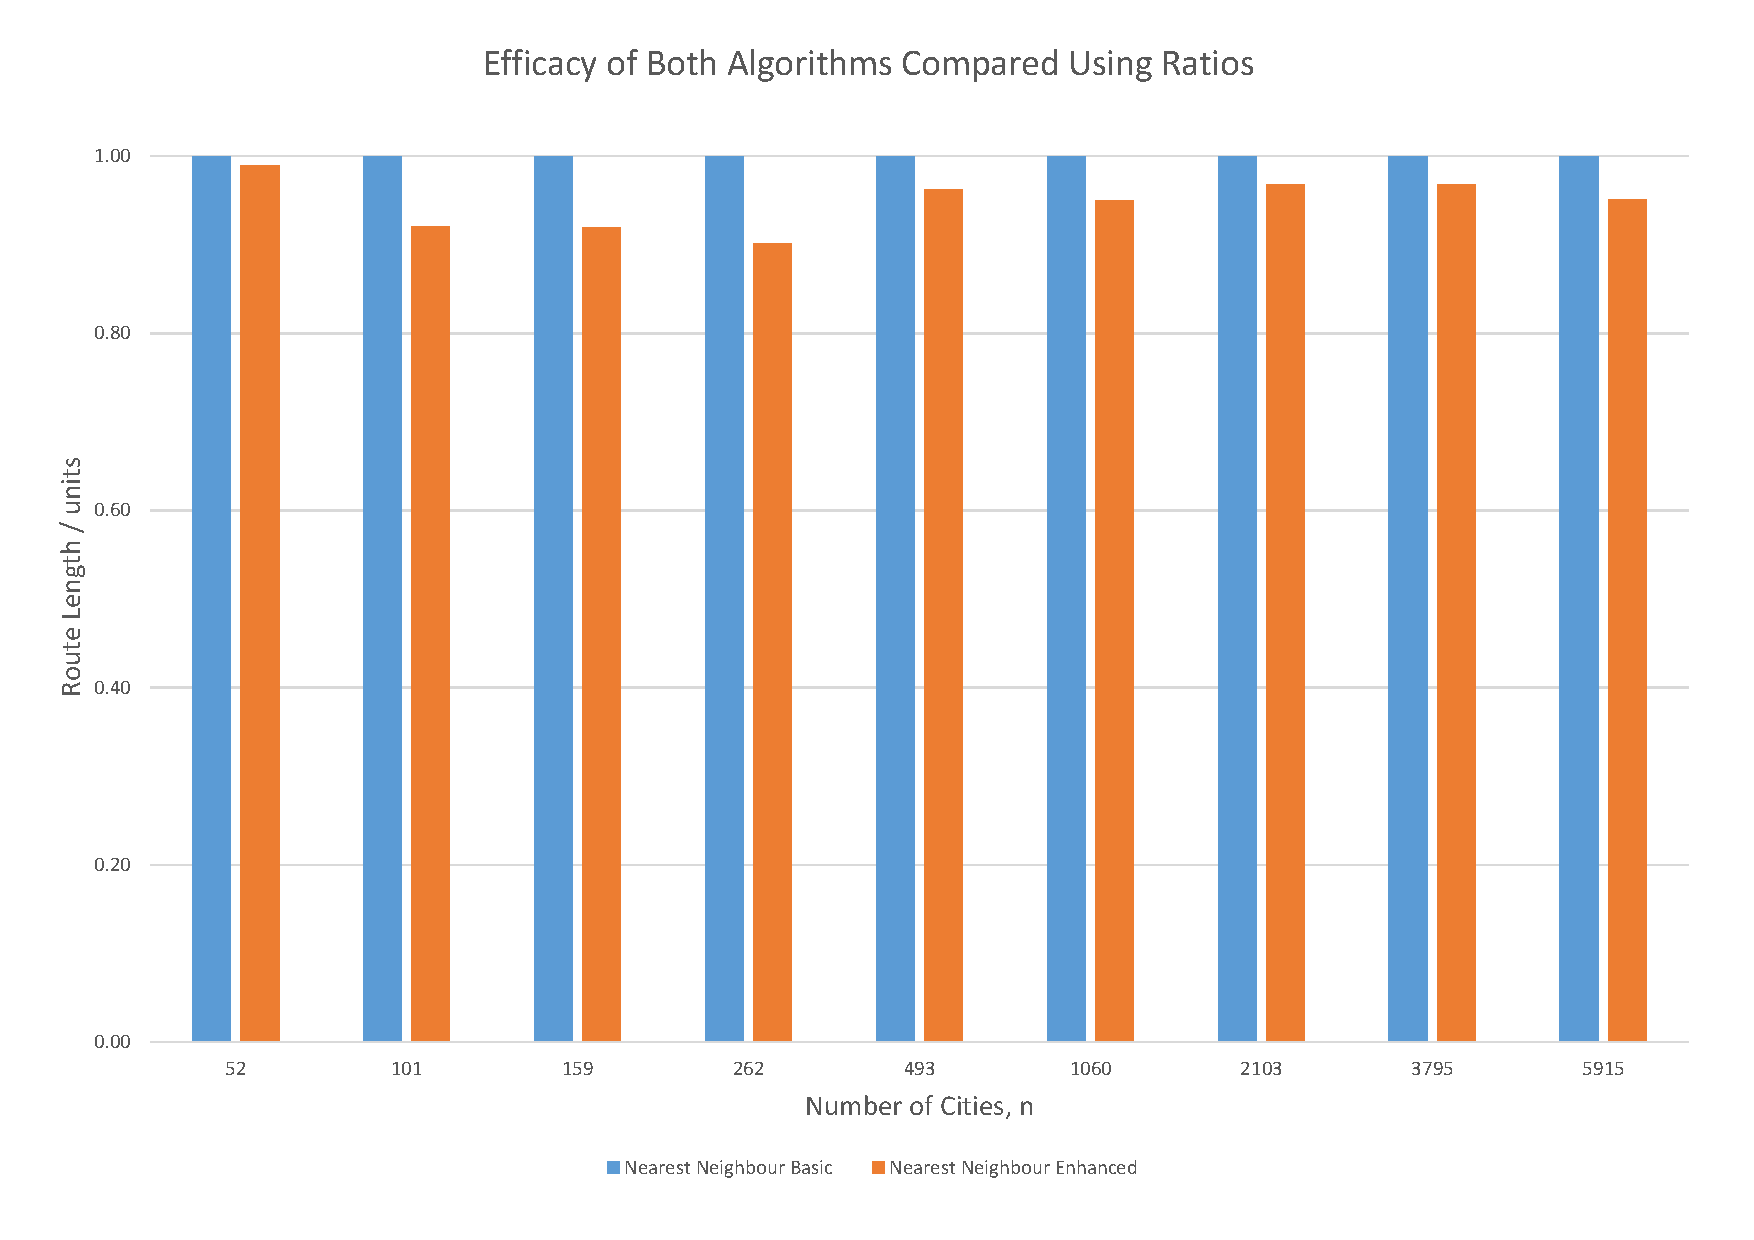
\includegraphics[width=\textwidth]{images/efficacy_compared_ratios.pdf}
	\clearpage
	\section{Efficiency of the Basic Algorithm}
		\label{efficiencybasicgraph}
		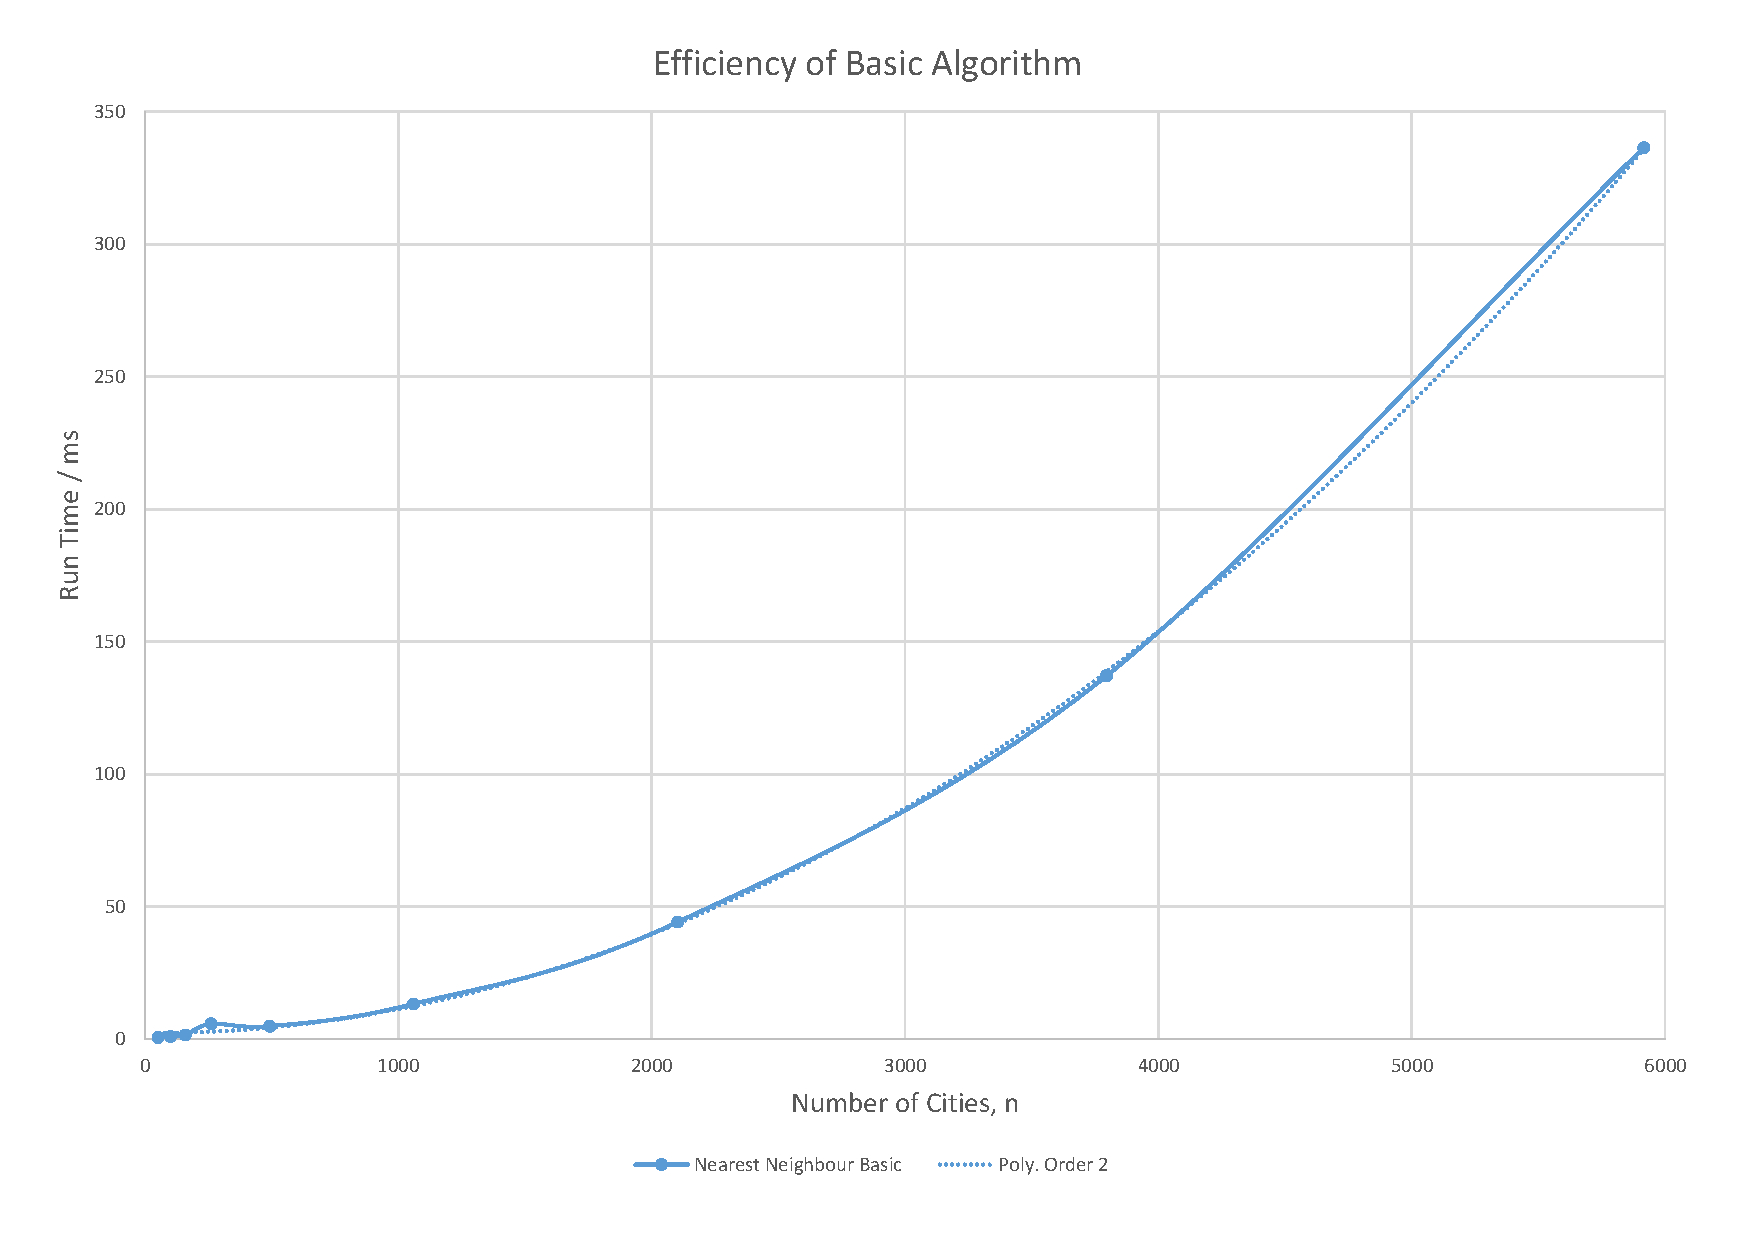
\includegraphics[width=\textwidth]{images/efficiency_basic.pdf}
	\clearpage
	\section{Efficiency of the Basic Algorithm}
		\label{efficiencyenhancedgraph}
		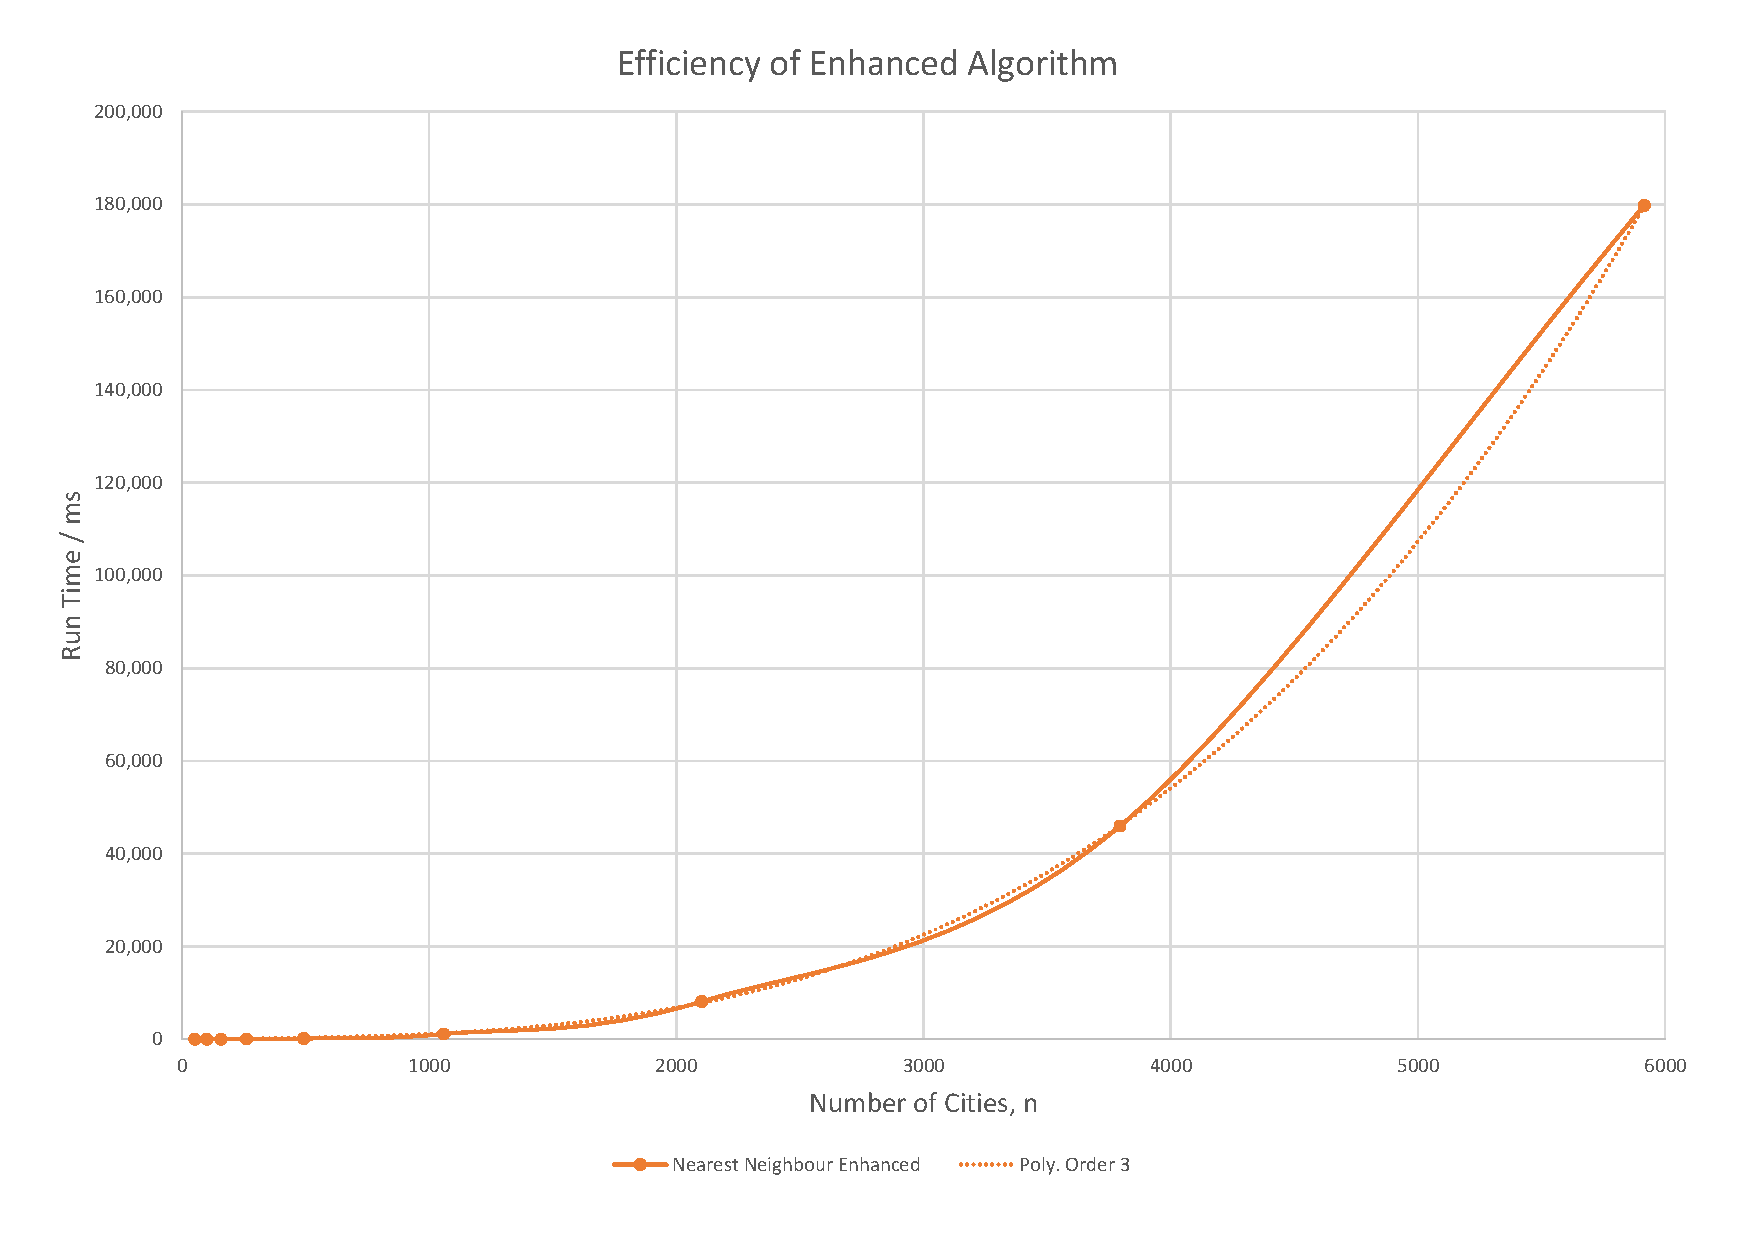
\includegraphics[width=\textwidth]{images/efficiency_enhanced.pdf}
	\clearpage
	\section{Efficiency of the Basic Algorithm}
		\label{efficiencycomparedgraph}
		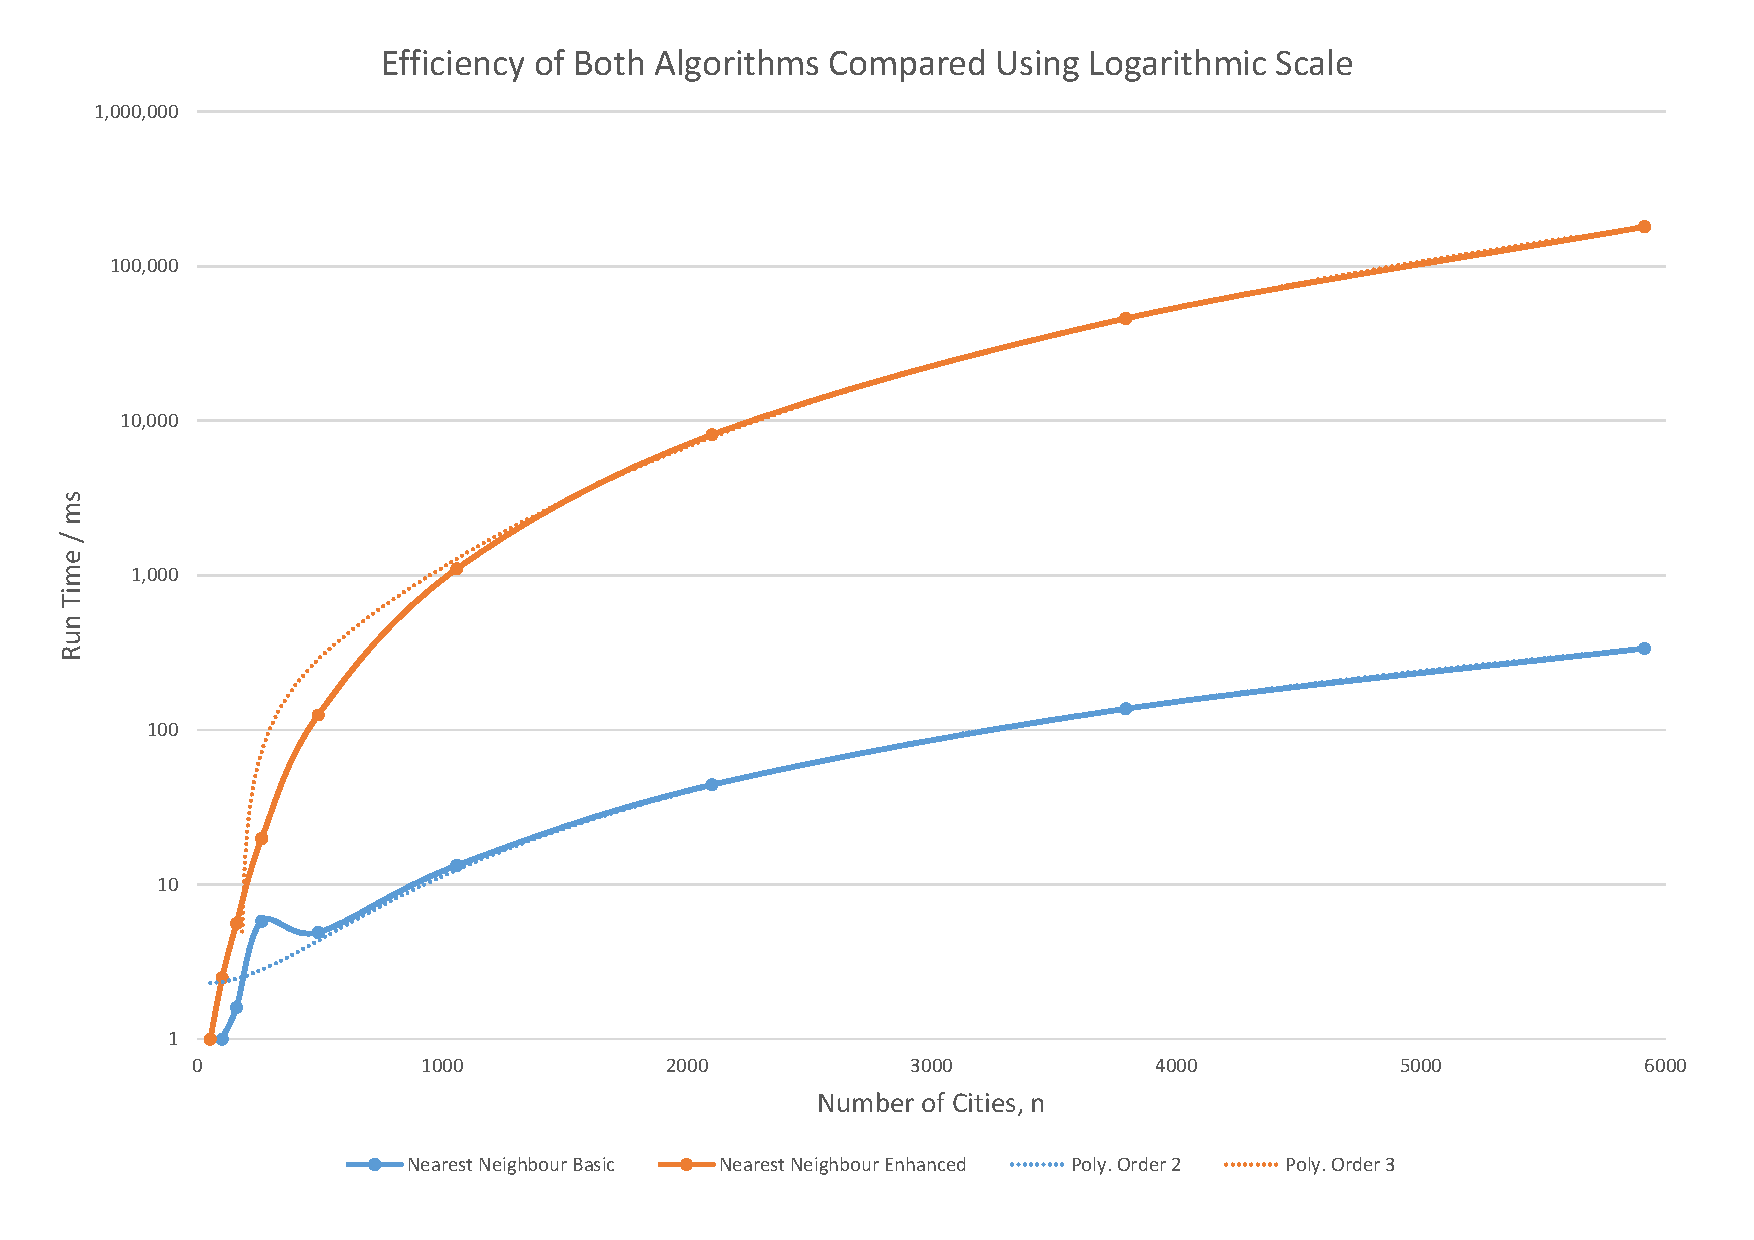
\includegraphics[width=\textwidth]{images/efficiency_compared.pdf}
	
	\clearpage
	\onecolumn
	\section{Main.java}
	\label{maincode}
	\begin{lstlisting}
	
		import java.awt.geom.Point2D;
		import java.util.ArrayList;
		import java.util.Random;
		
		public class Main {
		
			public static double routeLength(ArrayList<Point2D> cities){
				//Calculate the length of a TSP route held in an ArrayList as a set of Points
				double result=0;//Holds the route length
				Point2D prev = cities.get(cities.size()-1);
				//Set the previous city to the last city in the ArrayList as we need to measure the length of the entire loop
				for(Point2D city : cities){
					//Go through each city in turn
					result += city.distance(prev);
					//Get distance from the previous city
					prev = city;
					//Current city will be the previous city next time
				}
				return result;
			}
			
			public static double getDistance(Point2D currentCity, Point2D possible){
				//Calculate the distance between two points
				return Point2D.distance(currentCity.getX(), currentCity.getY(), possible.getX(), possible.getY());
			}
			
			public static ArrayList<Point2D> nearestNeighbourBasic(ArrayList<Point2D> cities){
				//Nearest Neighbour Basic algorithm
				ArrayList<Point2D> result = new ArrayList<Point2D>();
				Point2D closest = null;
				//Empty arraylist for results, empty point for closest city
				Point2D currentCity = cities.get(0);
				//Set the current city to the first city in the arraylist
				while (cities.size() > 0){\\
					//For all the cities, add the current city to the result and remove it from the cities list
					result.add(currentCity);
					cities.remove(currentCity);
					double distance = Double.POSITIVE_INFINITY;
					for (Point2D city : cities){
						//Go through each city to find which is closest to the current city
						if (getDistance(currentCity, city) < distance){
							closest = city;
							distance = getDistance(currentCity, city);
						}
					}
					currentCity = closest;
					//The closest city becomes the next current city
				}
				return result;
			}
			
			public static ArrayList<Point2D> nearestNeighbourRandomStart(ArrayList<Point2D> cities){
				//Nearest Neighbour Random Start algorithm
				ArrayList<Point2D> result = new ArrayList<Point2D>();
				Point2D closest = null;
				Random rn = new Random();
				int random = rn.nextInt(cities.size() + 1);
				//Empty arraylist for results, empty point for closest city, and a random number between 0 and n (n being the number of cities in the list)
				Point2D currentCity = cities.get(random);
				//Set the current city to a random city in the arraylist
				while (cities.size() > 0){
					//For all the cities, add the current city to the result and remove it from the cities list
					result.add(currentCity);
					cities.remove(currentCity);
					double distance = Double.POSITIVE_INFINITY;
					for (Point2D city : cities){
						//Go through each city to find which is closest to the current city
						if (getDistance(currentCity, city) < distance){
							closest = city;
							distance = getDistance(currentCity, city);
						}
					}
					currentCity = closest;
					//The closest city becomes the next current city
				}	
				return result;
			}
			
			public static ArrayList<Point2D> nearestNeighbourEnhanced(ArrayList<Point2D> cities){
				//Nearest Neighbour Enhanced algorithm
				ArrayList<Point2D> result = new ArrayList<Point2D>();
				ArrayList<ArrayList<Point2D>> sortedCitiesList = new ArrayList<ArrayList<Point2D>>();
				ArrayList<Double> lengths = new ArrayList<Double>();
				//Empty arraylist for results, empty arraylist of arraylists to store the sortedCities lists, empty arraylist for the lengths
				for (int i = 0; i < (cities.size()/10); i++){
					//For a tenth of the total number of cities, add a NNRandomStart sorted list to the arraylist of arraylists and get its length
					ArrayList<Point2D> tempCitiesList = new ArrayList<Point2D>(cities);
					sortedCitiesList.add(nearestNeighbourRandomStart(tempCitiesList));
					lengths.add(routeLength(sortedCitiesList.get(i)));
					//System.out.println("Length of route: " + lengths.get(i));
					double distance = Double.POSITIVE_INFINITY;
					if (lengths.get(i) < distance){
						//Determine the shortest length of all the routes stored in the arraylist of arraylists
						distance = lengths.get(i);
						result = sortedCitiesList.get(i);
					}
				}
				//System.out.println(distance);
				return result;
			}
			
			public static void main(String[] args) {
				//Loads in desired city file
				ArrayList<Point2D> cities = LibLoader.loadTSPLib("berlin52.tsp");
				//ArrayList<Point2D> cities = LibLoader.loadTSPLib("eil101.tsp");
				//ArrayList<Point2D> cities = LibLoader.loadTSPLib("u159.tsp");
				//ArrayList<Point2D> cities = LibLoader.loadTSPLib("gil262.tsp");
				//ArrayList<Point2D> cities = LibLoader.loadTSPLib("d493.tsp");
				//ArrayList<Point2D> cities = LibLoader.loadTSPLib("u1060.tsp");
				//ArrayList<Point2D> cities = LibLoader.loadTSPLib("d2103.tsp");
				//ArrayList<Point2D> cities = LibLoader.loadTSPLib("fl3795.tsp");
				//ArrayList<Point2D> cities = LibLoader.loadTSPLib("rl5915.tsp");
				
				//Print the number of cities for the file
				System.out.println("Number of cities in file: " + cities.size());
				
				// Start recording times
				final long startTime = System.currentTimeMillis();
				
				//Choose algorithm
				//ArrayList<Point2D> sortedCities = nearestNeighbourBasic(cities);
				ArrayList<Point2D> sortedCities = nearestNeighbourEnhanced(cities);
				
				//End recording time
				final long endTime = System.currentTimeMillis();			
				
				//Measure length of route found
				double length = routeLength(sortedCities);
				
				//Print results
				System.out.println("Route Length: " + length + "\nRun Time: " + (endTime - startTime) + "ms");
				
				//Print the number of cities for the file after the algorithm is run
				System.out.println("Number of cities in route: " + sortedCities.size());
			}
		}
	\end{lstlisting}
	
	\clearpage
	\section{LibLoader.java}
	\label{loadercode}
	\begin{lstlisting}
	
		import java.awt.geom.Point2D;
		import java.io.BufferedReader;
		import java.io.FileReader;
		import java.io.IOException;
		import java.util.ArrayList;
		
		public class LibLoader {
			
			public static ArrayList<Point2D> loadTSPLib(String fName){
				//Load in a TSPLib instance. This example assumes that the Edge weight type is EUC_2D.
				ArrayList<Point2D> result = new ArrayList<Point2D>();
				BufferedReader br = null;
				try {
					String currentLine;
					int dimension =0;//Hold the dimension of the problem
					boolean readingNodes = false;
					br = new BufferedReader(new FileReader(fName));
					while ((currentLine = br.readLine()) != null) {
						//Read the file until the end;
						if (currentLine.contains("EOF")){
							//EOF should be the last line
							readingNodes = false;
							//Finished reading nodes
							if (result.size() != dimension){
								//Check to see if the expected number of cities have been loaded
								System.out.println("Error loading cities");
								System.exit(-1);
							}
						}
						if (readingNodes){
							//If reading in the node data
							String[] tokens = currentLine.split(" ");
							//Split the line by spaces.
							float x = Float.parseFloat(tokens[1].trim());
							float y = Float.parseFloat(tokens[2].trim());
							Point2D city = new Point2D.Float(x,y);
							//Add this city into the arraylist
							result.add(city);
						}
						if (currentLine.contains("DIMENSION")){
							//Check the problem dimension (number of cities)
							String[] tokens = currentLine.split(":");
							dimension = Integer.parseInt(tokens[1].trim());
						}
						if (currentLine.contains("NODE_COORD_SECTION")){
							//Node data follows this line
							readingNodes = true;
						}
					}
				} catch (IOException e) {
				e.printStackTrace();
				} finally {
					try {
						if (br != null)br.close();
						} catch (IOException ex) {
						ex.printStackTrace();
						}
				}
				return result;
			}
		}
	\end{lstlisting}
\end{appendices}

\end{document}

